\subsection{Goal}
Nowadays programmers face the following situation when they try to optimize the memory performance of their programs: An access to a formerly unknown memory location is very expensive, it can take more than a 100 processor cycles to be completed. However, caches can reduce this time to under 10 cycles for a small subset of the memory. That means, while a programmer can not see that a cache is being used, it's very important to use it efficiently, the difference can make up 90\% of your computation time.\newline
To simplify this, a programmer needs tools. This specific tool we've developed is specialized on algorithms that work on two-dimensional matrices. It tries to visualize regions, access types and patterns so a programmer can decide which part of his algorithm is well-designed in regard to caches.

\subsection{Short description}
\subsubsection{Existing technical basis}
The operations aren't performed on the real cache but on a simulated, so that they can be traced. This will be done by more than one program: The tool McTracer, which is a Valgrind plugin, traces the operations. The simulated cache is represented by the program SimpleSim, which provides information if the operation was a hit or a miss. The task of our project was to modify the existing programs so that they can give us detailed data of the matrices like their size.
\\

We used the following programs:
\begin{itemize}
\item Valgrind
\item McTracer
\item SimpleSim
\item Examples (Multiplication, Jacobi, RedBlack)
\end{itemize}

\subsubsection{How this will be done?}
\begin{enumerate}
\item The tools analyze the cache usage
\item This information will be processed and the tools look for sequences and patterns
\item The program writes a file for the Java Application
\item The stand-alone Java GUI reads the file and produces a graphical output of the results
\end{enumerate}

\subsection{Terminology}
\begin{description}

\item[Debuggee]
	The piece of software for which we want to analyze cache usage. The term debuggee is used because it’s run with valgrind which is usually used for debugging.
\item[Matrix]
	A matrix is, in our case, an area of the memory which the debuggee has marked to contain data that is to be analyzed by our software. 
\item [Access]
	An access is an event generated for the debuggee. It marks loading or storing data to the main memory with a specific address.
\item[Relative Access]
	We are matching memory accesses to matrices and compute coordinates from that. For each access and it's previous access, a difference is coputed, and that is called a relative access. \newline
	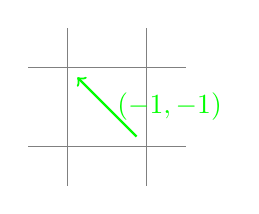
\begin{tikzpicture} %Tikzpictures are going to be fun. Our coordinate systems diverge...
		\draw [color=gray] (-0.5,-0.5) grid (1.5,1.5);
		\node (frst) at (1,0) {}; %nth access
		\node (scnd) at (0,1) {}; %n+1-th access
		\draw [->,color=green,thick] (frst) -- (scnd) node [midway,right,draw=none] {$(-1,-1)$};
	\end{tikzpicture}
\item[Pattern]
	A pattern is an ordered set of relative accesses. These accesses have been observed subsequently multiple (to be exact: at least two) times. It is not guaranteed that the first access of a pattern always occures first. Patterns can't tell you anything about when or in which compositions they occur
\item[Sequence]
	When scanning for patterns in the access stream, a series of consecutive accesses is often accounted to one pattern. The length of this series and what happens next is bundled into a sequence.
\end{description}


\subsection{Patterns and Sequences}
The idea behind patterns and sequences was to give a better insight into how the matrix is traversed.\newline
Consider the following example of accesses to a matrix:\newline
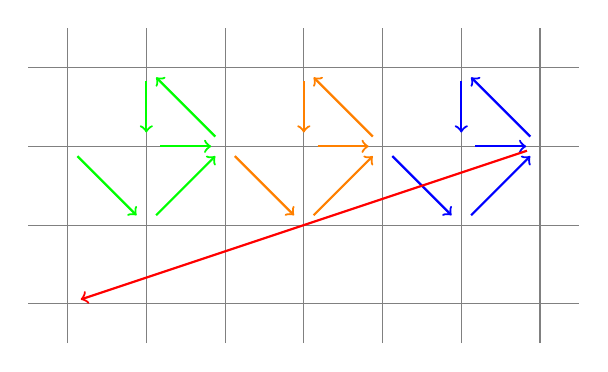
\begin{tikzpicture}
	\tikzstyle{accarrw} = [draw,->,thick, shorten <=5, shorten >=5]
	\draw [color=gray] (-0.5,-3.5) grid (6.5,0.5);
	\foreach \i/\c in {0/green, 1/orange, 2/blue} {
		\draw [accarrw,\c] ({0+\i*2},-1) -- ({1+\i*2},-2);
		\draw [accarrw,\c] ({1+\i*2},-2) -- ({2+\i*2},-1);
		\draw [accarrw,\c] ({2+\i*2},-1) -- ({1+\i*2},-0);
		\draw [accarrw,\c] ({1+\i*2},-0) -- ({1+\i*2},-1);
		\draw [accarrw,\c] ({1+\i*2},-1) -- ({2+\i*2},-1);
	}
	\draw [accarrw,red,bend left] (6,-1) -- (0,-3);
\end{tikzpicture}\newline
The green, orange and blue parts would each be considered an occurrence of the pattern (1,1),(1,-1),(-1,1),(0,1),(1,0). A pattern however does not know anything about which access is first or last, it only states that there is a short series of accesses that repeats.\newline
The three consecutive occurences of the pattern are considered a sequence. In this case, it's a sequence of length 3 with the next access (-6,2). The fact how often a sequence with these specifics is detected is counted by mctracer. Information that is not collected is; where the sequence was found (neither in terms of time or localization on the matrix) and which access of it's pattern was last (usually, it's the last access, but that isn't always certain).

